\section{Industry Use Cases}
\begin{frame}{}
    \LARGE Computer Vision: \textbf{Industry Use Cases}
\end{frame}

\begin{frame}[allowframebreaks]{Pipeline Corrosion \& Defect Analysis}
\begin{itemize}
    \item \textbf{CNN Architectures Used:}
    \begin{itemize}
        \item ResNet
        \item VGG
        \item InceptionNet
    \end{itemize}

    \item \textbf{Use Case:}
    \begin{itemize}
        \item Automated analysis of pipeline conditions using camera feeds.
        \item Classification of corrosion severity levels.
        \item Predictive maintenance through visual pattern recognition.
    \end{itemize}

    \begin{figure}
    \centering
    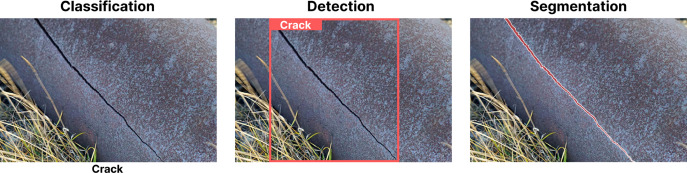
\includegraphics[width=0.8\linewidth]{images/cv-intro/Crack.jpg}
    \end{figure}
\end{itemize}

\framebreak

\begin{itemize}
    \item \textbf{Benefits:}
    \begin{itemize}
        \item Reduces manual inspection costs and time.
        \item Early detection prevents catastrophic failures.
        \item Enables data-driven maintenance scheduling.
    \end{itemize}

    \item \textbf{Links \& Resources:}
    \begin{itemize}
        \item \href{https://viso.ai/applications/computer-vision-in-oil-and-gas/}{viso.ai}
        \item \href{https://www.sciencedirect.com/science/article/pii/S2667143324000738}{ScienceDirect}
        \item \href{https://nextbrain.ca/top-10-real-world-use-cases-of-computer-vision-ai-in-the-oil-gas-industry/}{NextBrain}
    \end{itemize}
\end{itemize}
\end{frame}

\begin{frame}[allowframebreaks]{Equipment Defect Classification}
\begin{itemize}
    \item \textbf{CNN Architectures Used:}
    \begin{itemize}
        \item ResNet50 with Transfer Learning
        \item VGG19
        \item AlexNet
    \end{itemize}

    \item \textbf{Use Case:}
    \begin{itemize}
        \item Classify types of defects in steel surfaces and equipment.
        \item Automated quality control for manufactured components.
        \item Multi-class defect recognition (rust, cracks, deformation, etc.).
    \end{itemize}
\end{itemize}

\framebreak

\begin{figure}
    \centering
    \includegraphics[width=0.8\linewidth]{images/cv-intro/defect_classification.png}
\end{figure}

\begin{itemize}
    \item \textbf{Benefits:}
    \begin{itemize}
        \item 99.4\% accuracy with transfer learning approaches.
        \item Cost savings through early detection.
        \item Replaces subjective manual inspections.
    \end{itemize}

    \item \textbf{Links \& Resources:}
    \begin{itemize}
        \item \href{https://www.mdpi.com/2076-3417/13/9/5260}{MDPI: Steel defect detection (ResNet, 99.4\% accuracy)}
    \end{itemize}
\end{itemize}
\end{frame}

\begin{frame}[allowframebreaks]{Oil Spill Detection \& Classification}
\begin{itemize}
    \item \textbf{CNN Architectures Used:}
    \begin{itemize}
        \item YOLOv4
        \item Mask R-CNN
        \item CNNs
    \end{itemize}

    \item \textbf{Use Case:}
    \begin{itemize}
        \item Classify oil spill severity and type from SAR/optical imagery.
        \item Automated environmental monitoring systems.
        \item Multi-class classification for response prioritization.
    \end{itemize}
\end{itemize}

\begin{figure}
    \centering
    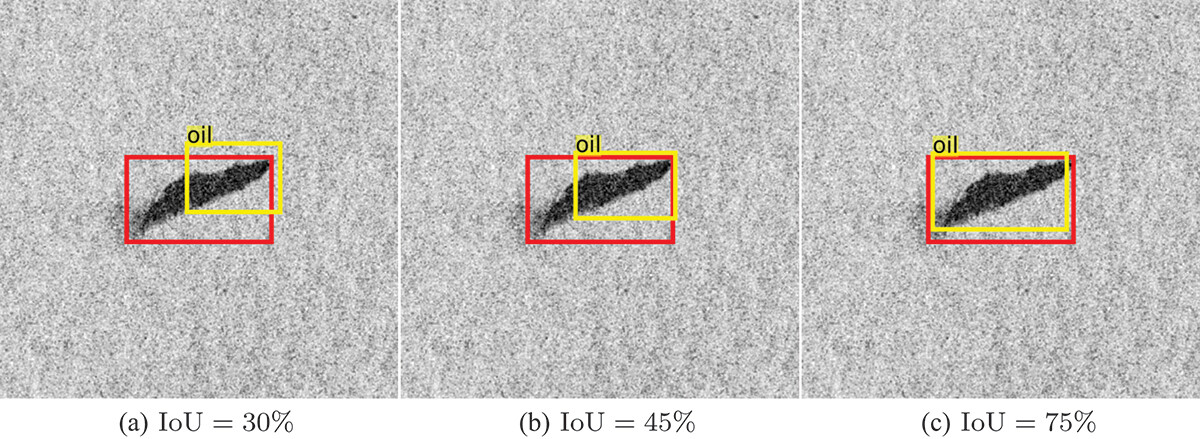
\includegraphics[width=0.8\linewidth]{images/cv-intro/oil_spills.jpg}
\end{figure}

\begin{itemize}
    \item \textbf{Benefits:}
    \begin{itemize}
        \item Faster emergency response decisions.
        \item Accurate spill characterization for cleanup planning.
        \item Compliance with environmental regulations.
    \end{itemize}

    \item \textbf{Research Papers \& Resources:}
    \begin{itemize}
        \item \href{https://www.tandfonline.com/doi/full/10.1080/01431161.2022.2109445}{Deep learning oil spill detector (Sentinel-1 SAR, 2022)}
        \item \href{https://www.sciencedirect.com/science/article/pii/S2667143324000738}{Comprehensive review of oil spill DL methods (2024)}
    \end{itemize}
\end{itemize}
\end{frame}
